% ============================================================
%  SENTINEL-GNSS — General Team Poster  (A1 Portrait, 594×841mm)
%  Compile: pdflatex (no bibtex needed — citations inline)
%
%  Uses only standard LaTeX packages (MiKTeX compatible).
%  Font size is scaled to A1 using 'a1paper' geometry + large base font.
% ============================================================
\documentclass[20pt]{extarticle}   % extarticle supports large base font sizes

\usepackage[T1]{fontenc}
\usepackage[utf8]{inputenc}
\usepackage{lmodern}

% A1 paper, portrait
\usepackage[a1paper,landscape=false,
            top=1.8cm,bottom=1.8cm,left=2cm,right=2cm]{geometry}

\usepackage{multicol}
\setlength{\columnsep}{1.4cm}
\usepackage{amsmath,amssymb}
\usepackage{graphicx}
\usepackage{booktabs}
\usepackage{array}
\usepackage{float}
\usepackage{caption}
\captionsetup{font=large,labelfont=bf}
\usepackage[dvipsnames]{xcolor}
\definecolor{buaaBlue}{RGB}{0,91,172}
\definecolor{buaaNavy}{RGB}{0,51,102}
\definecolor{buaaSky}{RGB}{0,160,233}
\definecolor{cleanGreen}{RGB}{76,175,80}
\definecolor{warnOrange}{RGB}{255,152,0}
\definecolor{degradRed}{RGB}{244,67,54}
\definecolor{blockBG}{RGB}{235,244,252}

\usepackage{tcolorbox}
\tcbuselibrary{skins,breakable}
\usepackage{mdframed}
\usepackage{parskip}
\setlength{\parskip}{6pt}
\usepackage{enumitem}
\setlist[itemize]{noitemsep,topsep=2pt}

% ---- Coloured section boxes ----
\newmdenv[
  backgroundcolor=blockBG,
  linecolor=buaaBlue,
  linewidth=2pt,
  roundcorner=6pt,
  innertopmargin=8pt,
  innerbottommargin=8pt,
  innerleftmargin=10pt,
  innerrightmargin=10pt,
  skipabove=6pt,
  skipbelow=6pt
]{poblock}

\newcommand{\posec}[1]{%
  \vspace{4pt}
  {\large\bfseries\color{buaaNavy}#1}\\[-4pt]
  {\color{buaaBlue}\rule{\linewidth}{1.5pt}}
  \vspace{4pt}
}

\newcommand{\clean}[1]{\textcolor{cleanGreen}{\textbf{#1}}}
\newcommand{\warn}[1]{\textcolor{warnOrange}{\textbf{#1}}}
\newcommand{\degrad}[1]{\textcolor{degradRed}{\textbf{#1}}}

\pagestyle{empty}

\begin{document}

% ================================================================
%  HEADER BANNER
% ================================================================
\noindent
\begin{tcolorbox}[
  colback=buaaNavy, colframe=buaaNavy,
  boxrule=0pt, arc=8pt,
  left=16pt, right=16pt, top=10pt, bottom=10pt
]
  \begin{center}
    {\fontsize{52}{60}\bfseries\color{white} SENTINEL-GNSS}\\[6pt]
    {\fontsize{28}{34}\color{buaaSky}
     Proactive Multi-Horizon Prediction of GNSS Signal Degradation\\
     for Autonomous Vehicle Navigation}\\[8pt]
    {\large\color{white}
     \textbf{Ojerinde Joel} (LS2525253) \quad
     \textbf{Ogunlade Joshua} (LS2525237) \quad
     \textbf{Mustapha Ibrahim} (LS2525238) \quad
     \textbf{Ingeriyinkindi Claudine} (LS2525236) \quad
     \textbf{Rashid Md Harun Or} (LS2525219)}\\[4pt]
    {\normalsize\color{white!70!buaaSky}
     Hangzhou International Institute of Innovation (H3I) · Beihang University · Hangzhou 2026}
  \end{center}
\end{tcolorbox}

\vspace{0.6cm}

% ================================================================
%  THREE-COLUMN BODY
% ================================================================
\begin{multicols}{3}

% ---- COLUMN 1 ----

\posec{1. The Problem}

\begin{poblock}
Autonomous vehicles at 60\,km/h travel \textbf{17 metres every second}.
GNSS—the sole source of drift-free absolute position—fails silently in urban canyons:
buildings reflect or block satellite signals, producing positioning errors of
\textbf{10–200\,m} with no external indication.

\medskip
\textbf{Every existing monitor is reactive.} RTKLIB quality codes, RAIM, and recent
ML classifiers report degradation \emph{at the moment it happens}, giving the vehicle
\textbf{zero} preparation time.

\medskip
\textbf{We ask: can degradation be predicted 5–30 seconds before it occurs?}
\end{poblock}

\begin{center}
  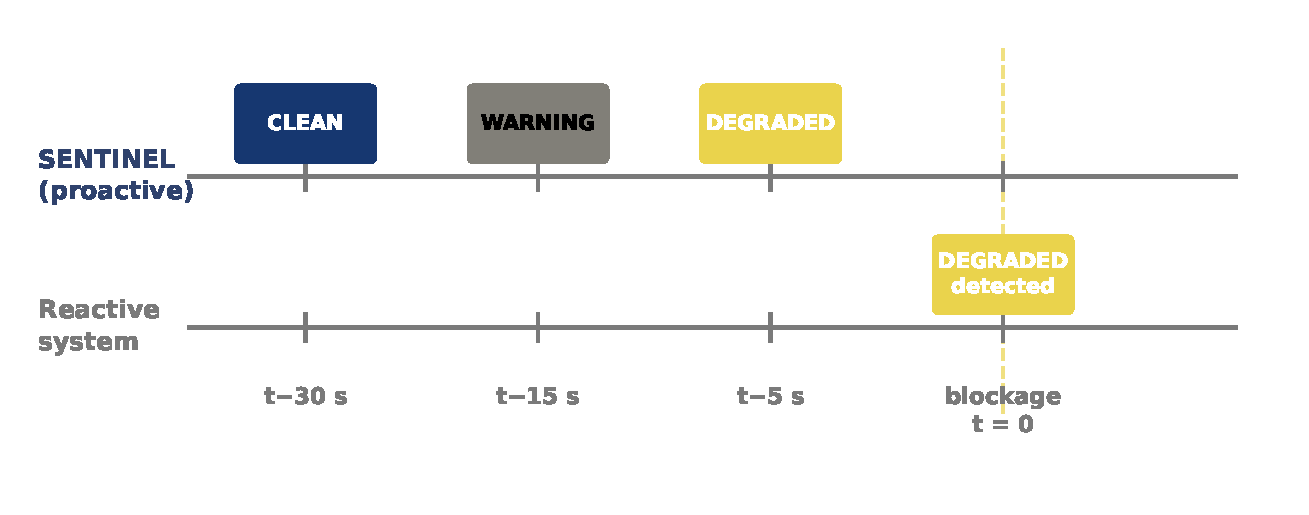
\includegraphics[width=0.9\columnwidth]{../../results/paper_figures/fig13_reactive_vs_proactive.pdf}
  \captionof{figure}{Reactive vs.\ proactive degradation warning.
  SENTINEL raises WARNING before the vehicle enters the NLOS zone.}
\end{center}

\posec{2. What a Warning Buys}

\begin{poblock}
\begin{tabular}{lll}
  \toprule
  Horizon & Distance & Vehicle action \\
  \midrule
  +5\,s  & 83\,m  & Tighten IMU fusion, slow down \\
  +15\,s & 250\,m & Pre-engage dead-reckoning \\
  +30\,s & 500\,m & Re-route to avoid NLOS zone \\
  \bottomrule
\end{tabular}
\end{poblock}

\posec{3. Dataset}

\begin{poblock}
\textbf{149,662 labelled epochs} · 4 cities · 9+ receiver types
\begin{itemize}
  \item Beihang campus (Scenarios A–E): controlled blockage scenarios
  \item UrbanNav Hong Kong: urban canyons, tunnels, open roads
  \item \textbf{Tokyo (held out):} Shinjuku + Odaiba — never seen during training
\end{itemize}
\textbf{3-class labels:} \clean{CLEAN} / \warn{WARNING} / \degrad{DEGRADED}\\
\textbf{37 features/epoch} in 7 groups: position, signal strength, satellite geometry,
pseudorange, temporal, atmospheric, receiver status
\end{poblock}

\begin{center}
  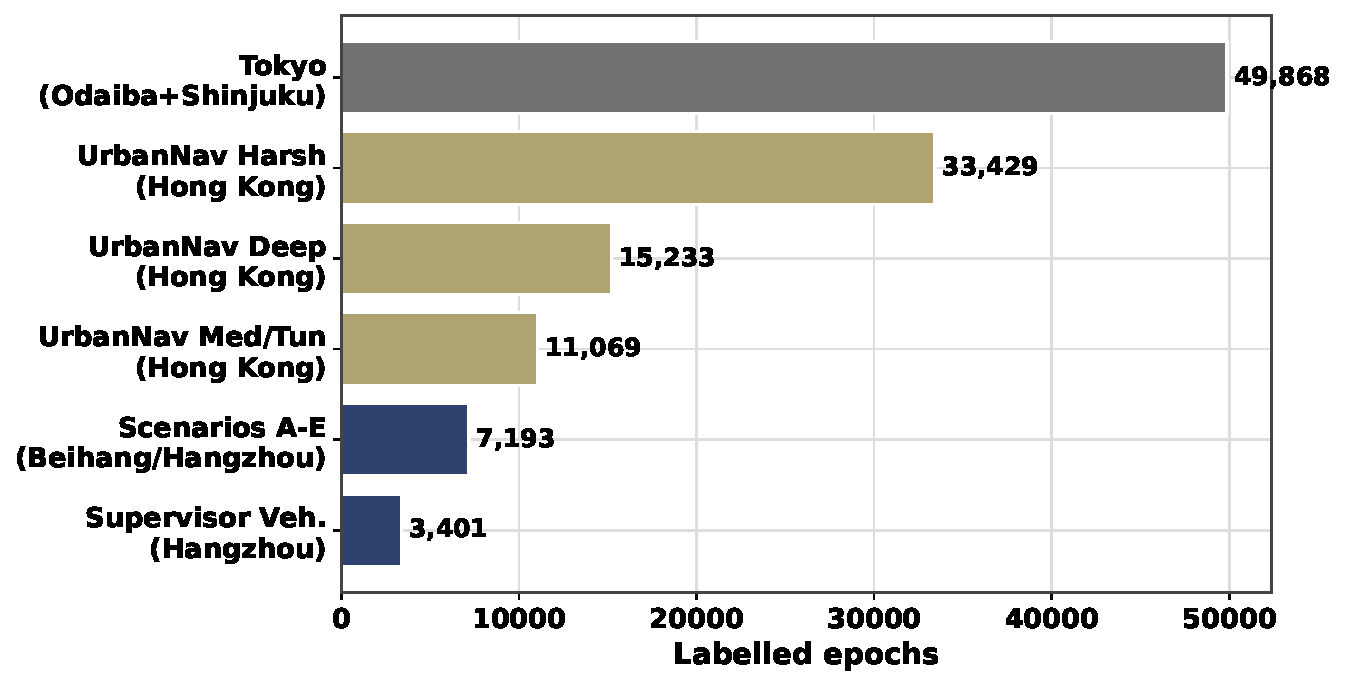
\includegraphics[width=0.9\columnwidth]{../../results/paper_figures/fig10_dataset_composition.pdf}
  \captionof{figure}{Dataset composition by city and receiver type.}
\end{center}

% ---- COLUMN 2 ----

\posec{4. SENTINEL-GNSS Architecture}

\begin{poblock}
\textbf{Hybrid Transformer + LSTM} (1.46\,M parameters)

\begin{itemize}
  \item \textbf{Transformer encoder} (2 layers, 8 heads, $d=128$):
    captures global satellite-geometry trends across the 30-second window
  \item \textbf{LSTM} (2 layers, hidden 256):
    captures sequential approach dynamics (gradual C/N$_0$ decline)
  \item \textbf{Four output heads:} $+5$\,s, $+15$\,s, $+30$\,s + auxiliary $t{+}0$
  \item \textbf{Training:} Focal loss ($\gamma=1.0$), class weights $[1,2,5]$,
    AdamW, cosine annealing
\end{itemize}
\end{poblock}

\begin{center}
  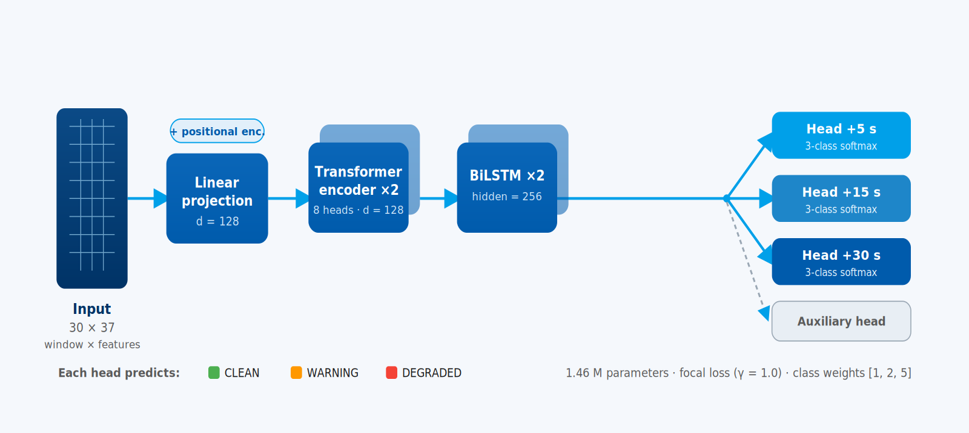
\includegraphics[width=0.92\columnwidth]{../../report/sentinel_gnss_inside.png}
  \captionof{figure}{SENTINEL architecture: one forward pass produces all three prediction horizons.}
\end{center}

\posec{5. Classification Results}

\begin{poblock}
\begin{tabular}{lccc}
  \toprule
  Horizon & Macro-F1 & MCC & DEG F1 \\
  \midrule
  \textbf{+5\,s}  & \textbf{0.821} & 0.773 & \textbf{0.718} \\
  +15\,s & 0.741 & 0.691 & 0.583 \\
  +30\,s & 0.783 & 0.731 & 0.629 \\
  \bottomrule
\end{tabular}

\medskip
\degrad{DEGRADED recall at +5\,s: \textbf{0.847}} —
catches 85\,\% of impending degradations 5 seconds early.

\medskip
\textbf{9.46$\times$ faster} than three separate tree models; 0.0449\,ms/sample.
\end{poblock}

\begin{center}
  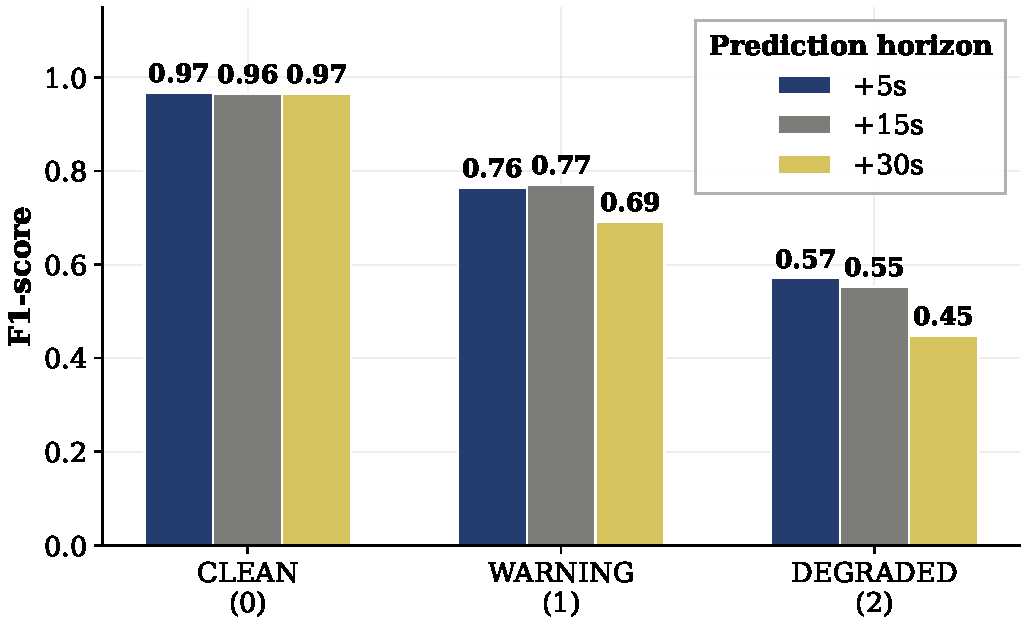
\includegraphics[width=\columnwidth]{../../results/paper_figures/multi_horizon_comparison.pdf}
  \captionof{figure}{Multi-horizon Macro-F1 and per-class F1.
  The +5\,s horizon is used for real-time EKF integration.}
\end{center}

% ---- COLUMN 3 ----

\posec{6. Cross-City Generalisation}

\begin{poblock}
Trained on Beihang + Hong Kong; tested on \textbf{Tokyo — never seen}.

\begin{tabular}{lcc}
  \toprule
  Model & Tokyo Macro-F1 & Tokyo DEG F1 \\
  \midrule
  \textbf{SENTINEL (DL)} & 0.649 & \textbf{\textcolor{cleanGreen}{0.75}} \\
  RandomForest            & 0.618 & \textbf{\textcolor{degradRed}{0.15}} \\
  \bottomrule
\end{tabular}

\medskip
\textbf{5$\times$ difference} in Tokyo DEGRADED F1.
Trees memorise city-specific thresholds; SENTINEL learns transferable degradation
representations.
\end{poblock}

\begin{center}
  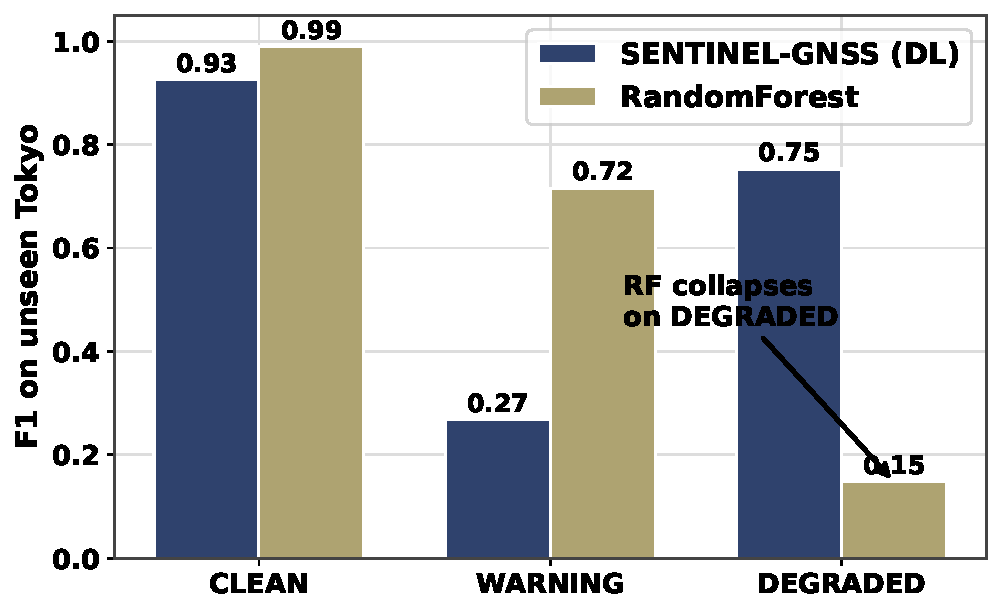
\includegraphics[width=0.88\columnwidth]{../../results/paper_figures/fig05_crosscity_degraded.pdf}
  \captionof{figure}{Cross-city DEGRADED F1: DL transfers, RF collapses.}
\end{center}

\posec{7. Prediction-Informed EKF Fusion}

\begin{poblock}
SENTINEL +5\,s prediction inflates GPS measurement noise covariance
\emph{before} bad measurements arrive:

\[
  \mathbf{R} = \begin{cases}
    (40\,\mathrm{m})^2 \mathbf{I} & P(\text{DEG}) > 0.45 \\
    r_\mathrm{base}^2 \mathbf{I}  & \text{otherwise}
  \end{cases}
\]

Also evaluated: \textbf{Huber robust EKF} (IRLS downweighting) and
\textbf{Bootstrap PF} (Student-$t$ GPS likelihood, N=500 particles).

\medskip
\begin{tabular}{lcc}
  \toprule
  Method / Scenario & Deg. RMSE & Gain \\
  \midrule
  EKF Fixed-R (Trimble) & 24.3\,m & \textbf{+48.8\,\%} \\
  SENTINEL+online (Trimble) & 26.9\,m & \textbf{+43.2\,\%} \\
  Huber EKF (u-blox)    & 58.6\,m & \textbf{+25.2\,\%} \\
  PF Student-$t$ (Odaiba) & 35.4\,m & \textbf{+40.1\,\%} \\
  \bottomrule
\end{tabular}
\end{poblock}

\begin{center}
  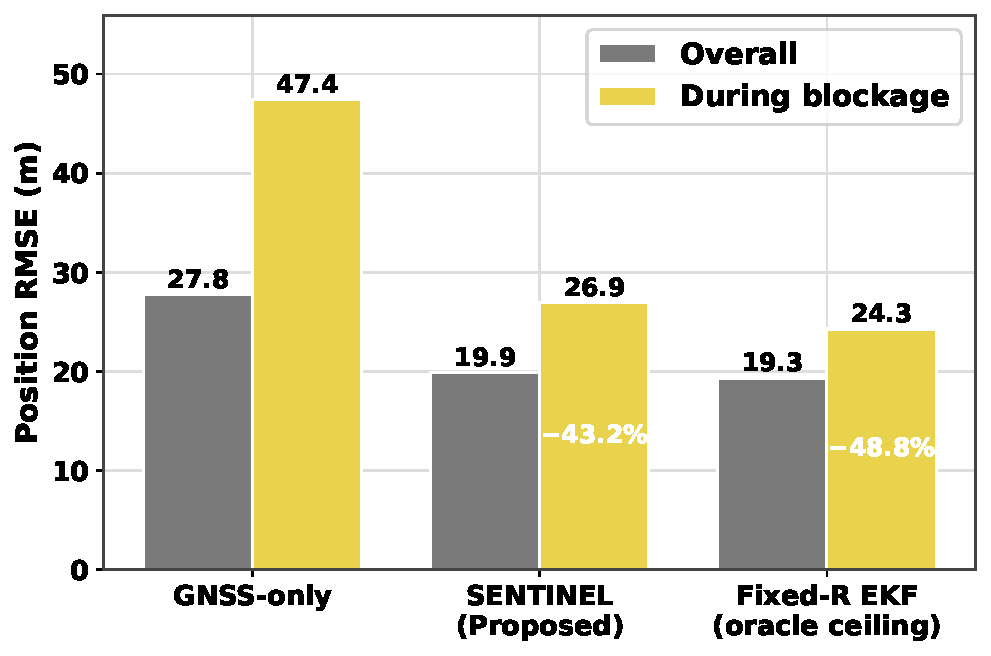
\includegraphics[width=0.92\columnwidth]{../../results/paper_figures/fig07_ekf_rmse.pdf}
  \captionof{figure}{Degraded-segment RMSE: all methods × all scenarios.
  No single method dominates — environment-aware selection matters.}
\end{center}

\posec{8. Conclusions}

\begin{poblock}
\begin{itemize}
  \item GNSS degradation is \textbf{predictable 5–30\,s in advance}
    with Macro-F1\,=\,0.821 at the actionable +5\,s horizon
  \item The hybrid Transformer-LSTM \textbf{transfers across cities};
    classical ML does not (5$\times$ DEGRADED F1 gap on Tokyo)
  \item Prediction-informed EKF fusion reduces degraded positioning RMSE
    by \textbf{up to 48.8\,\%} in real Tokyo urban drives
  \item Environment-aware method selection: Fixed-R EKF (clean GPS),
    Huber EKF (heavy-tailed), Student-$t$ PF (random NLOS)
\end{itemize}

\medskip
\textbf{Code:} {\small\texttt{github.com/Jorshuare/\allowbreak AI-Based-\allowbreak Prediction-\allowbreak for-GNSS-\allowbreak Signal-\allowbreak Degradation}}
\end{poblock}

\end{multicols}

% ================================================================
%  FOOTER
% ================================================================
\noindent
{\color{buaaBlue}\rule{\linewidth}{1.5pt}}\\[3pt]
\begin{center}
  {\small\color{buaaNavy}
   \textbf{Contact:} joelojerinde@gmail.com \quad
   \textbf{Institution:} H3I, Beihang University, Hangzhou, China \quad
   \textbf{Year:} 2026}
\end{center}

\end{document}
